\documentclass[12pt,a4paper]{report}

% Pacotes para acentuação e formatação
\usepackage[utf8]{inputenc}
\usepackage[T1]{fontenc}
\usepackage[brazil]{babel}
\usepackage{setspace}    % Para espaçamento
\usepackage{lipsum}      % Texto de exemplo (remova se não precisar)
\usepackage{graphicx}

\begin{document}
	
	% ----------- CAPA -----------
	\begin{titlepage}
		\centering
		\vspace*{5cm} % Espaço do topo
		
		{\Huge\bfseries Arquitetura de Computadores I\par} % Título
		
		\vspace{0.5cm}
		{\Large 2025/2\par} % Ano
		
		\vfill
		{\large Nicolas Ramos Carreira\par} % Nome
		
		\vspace*{2cm}
	\end{titlepage}
	
	% ----------- SUMÁRIO -----------
	\tableofcontents
	\newpage
	
	% ----------- CONTEÚDO -----------
	\chapter{Importância da matéria}
	Esta é sem dúvidas uma das disciplinas mais importantes para um Cientista da Computação, pois sem ela:
	
	\begin{itemize}
		\item Não saberemos como o computador funciona de fato
		\item Não seremos programadores tão bons como podemos ser
		\item Seremos mais sucessetiveis a cometer determinados erros
		
	\end{itemize}
	% Exemplo com texto fictício:
	%\lipsum[1]
	
	\chapter{O que aprenderemos}
	\section{Computadores são burros para fazer cálculos}
	\subsection{A conta: (43,1 - 43,2) + 1}
	\subsection{Propriedades matemáticas}
	\section{Como o Software roda no Hardware}
	
	\section{A memória}
	\subsection{O que é de fato?}
	Muitos programas dependem basicamente da memória RAM, mas a memória RAM não existe, é uma abstração limitada. O que existe é um complexo
	sistema hierárquico de memórias diferentes.
	
	Um exemplo disso é que temos a memória "Registradora", que se encontra no topo da hierarquia. Ela é a memória mais rápida que existe e que roda na mesma velocidade da CPU (ela fica dentro da CPU).
	
	Além disso, temos as memórias cach, que dão suporte a memória registradora.
	
	\begin{center}

		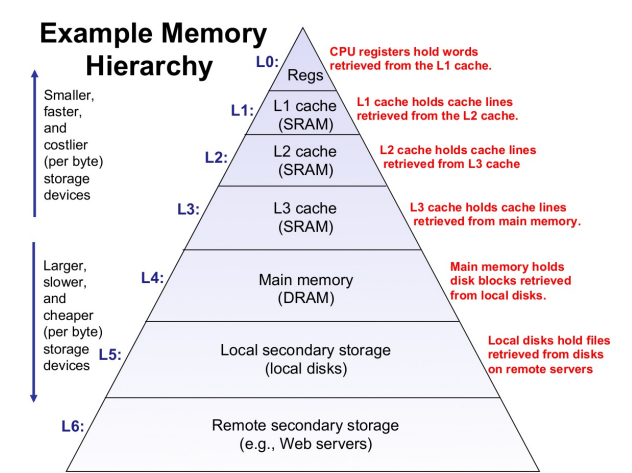
\includegraphics[width=8cm,height=5cm,keepaspectratio=false]{imagens-teoria/hierarquia_memoria.png}
		
	\end{center}
	
	\subsection{Bugs no referenciamento de memória são perniciosos}
	Quando estamos fazendo nosso programa, poderemos nos deparar com bugs de memória. Esses bugs podem ser bastante trabalhosos e chatos de lidar. Isso porque são bugs dificeis de serem debuggados
	\subsection{O porquê entender}
	Dado o contexto anterior, para ser um bom programador, você precisará entender a representação em nível de máquina, na memória, das estruturas de dados e como elas funcionam, pois isso faz uma grande diferença na sua habilidade de evitar e lidar com problemas de referenciamento de memória e vulnerabilidades no seu programa.
	
	Sendo assim, precisaremos entender:
	\begin{itemize}
		\item A hierarquia de memória
		\item Como a arquitetura da memória
		e linguagens como C podem levar a bugs de referenciamento de memória que são complicados de debugar e que podem ser distantes do tempo e espaço
		\item Que a performance da memória
		não é uniforme e que é necessário otimizar
		para o baixo nível também
	\end{itemize}  
	
	\section{Insight sobre abstrações}
	Boa parte do que sabemos sobre os computadores são, na verdade abstrações. No mais baixo nível possível, para o computador realizar uma soma, ele move eletrons.
	
	Sabendo disso, ao longo do tempo, nós fomos precisando de abstrações para representar isso. Foi então que vieram os componentes eletronicos. Porém nós ainda não conseguimos programar/interagir com isso. Dessa forma, abstrairam mais e criaram os circuitos elétricos analogicos. Ainda assim, não conseguimos programar/interagir bem com isso, então criaram a abstração dos circuitos digitais (0, 1, portas lógicas).
	
	\chapter{Introdução}
	\section{Acerca da história}
	
	Ao longo da história, nós tivemos algumas revoluções:
	
	\begin{itemize}
		\item Revolução agricola: O homem aprendeu a plantar
		\item Revolução industrial: Surgiram os trabalhos remunerados em grande escala
		\item Revolução da computação/informação: É a revolução que estamos tendo hoje. A partir dela:
		\begin{itemize}
			\item Conhecemos o DNA humano e de outras especies base por base (por conta do surgimento de grandes bancos de dados e aumento de poder computacional)
			\item Surgimento de carros autonomos
			\item Surgimento dos celulares
			\item Surgimento da internet
			\item Surgimento dos buscadores (google..)
		\end{itemize}
	\end{itemize}
	
	E no futuro? Bom não sabemos, mas uma coisa é certa. As evoluções que foram possíveis dentro da computação graças ao aumento do poder de processamento dos processadores e é o que vamos ver na próxima seção
	
	\section{Lei de moore, computadores e performance}
	
	\subsection{A lei de moore e algumas pills}
	
	Segundo a lei de Moore, o poder de processamento aumentava em 2x a cada dois anos, mantendo o custo.
	
	\begin{center}
		
		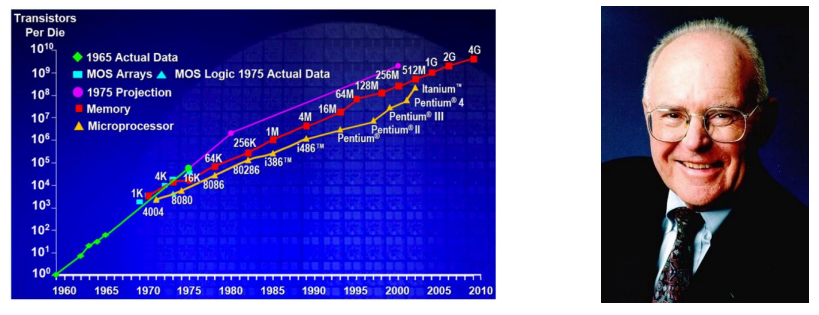
\includegraphics[width=14cm,height=5cm,keepaspectratio=false]{imagens-teoria/moore.png}
		
	\end{center}
	
	
	Foi esse aumento do poder de processamento que como dissémos na seção anterior, possibilitou essa grande evolução dentro da computação. No entanto, essa lei por muito tempo também salvou os programadores ruins, uma vez que seu programa poderia ser muito ruim, que a cada dois anos ele iria rodar mais rápido.
	
	A lei de Moore foi possibilitada graças a miniaturização dos transistors. Algo engraçado é que nos dias de hoje os transistors estão na faixa dos 7 nanometros e essa é a barreira fisica que chegamos, ou seja, não conseguimos mais diminui-los. Chegamos a essa barreira em 2018.
	
	Isso, logicamente, causou um panico nos programadores ruins, pois ou ele faz um código bem otimizado ou ele terá que aprender a fazer programação em paralelo (até mesmo os bons programadores precisam aprender programação em paralelo)
	
	\subsection{As classes de computadores}
	
	Os computadores podem ser diferenciados em algumas classes. Elas são: Computadores pessoais, servidores, super computadores e sistemas embarcados. Vamos ver algumas informações sobre eles: 
	
	\begin{itemize}
		\item Computadores pessoais: São computadores de uso geral (destinado a varias atividades) e são baseados em um equilibrio entre custo e performance
	\end{itemize}
	
	\begin{center}
		
		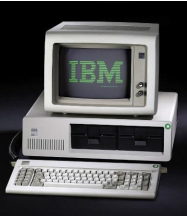
\includegraphics[width=8cm,height=5cm,keepaspectratio=false]{imagens-teoria/comp_geral.png}
		
	\end{center}
	
	\begin{itemize}
		\item Servidores: São computadores usados para acesso em rede. Eles possuem alta capacidade, alta performance e alta confiabilidade
	\end{itemize}
	
	\begin{itemize}
		\item Supercomputadores: São computadores que possuem aplicações cientificas e de engenharia de alta complexidade
	\end{itemize}
	
	\begin{itemize}
		\item Sistemas embarcados: Ficam dentro de dispositivos de hardware. São limitados. A ideia é fazer uma coisa só e bem feita, sem errar.
	\end{itemize}
	
	Agora uma curiosidade é que o maior número de computadores no mundo são sistemas embarcados. A ideia da disciplina de arquitetura de computadores além de falar sobre a arquitetura dos computadores é trabalhar com sistemas embarcados justamente pelo motivo deles se fazerem extremamente presente
	
	
	\subsection{A perfomance}
	Sabemos que a perfomance dependerá do hardware de da própria aplicação, uma vez que:
	
	\begin{itemize}
		\item Depende do algoritmo (Big-O)
		\item Depende da Linguagem de programação (sistemas de alta performance devem ser escritos em C e C++)
		\item Depende de Sistema de entrada e saída do computador
		\item Depende de processador e memória, que determinam o quão rápido instruções podem ser executadas 
	\end{itemize}
	
	\subsection{As 7 grandes ideias}
	A evolução da computação pode ser resumida em 7 grandes ideias. Sao elas:
	
	\begin{enumerate}
		\item Abstrações: Humanidade criou diversas abstrações, uma vez que o computador é apenas a passagem de energia. Bits são apenas abstrações, nós falamos que tem 0 e 1 no HD, mas o que tem é um campo magnético voltado para cima e para baixo
		\item Performance do caso comum:
		\item Performance do paralelismo
		\item Performance do pipelining
		\item Performance por predição:
		\item Hierarquia de memorias
		\item Confiança por redundancia
	\end{enumerate}
	
	
	Existia uma oitava ideia, que era a lei de Moore, mas sabemos que ela morreu pelos motivos que falamos na seção "A lei de moore e algumas pills"
	
	
	\section{Falando sobre software}
	
	Quando falamos sobre software, na verdade, podemos estar nos referindo a diferentes tipos de software
	
	\begin{itemize}
		\item Software aplicativo: Aquilo que fazemos (Hello World e etc)
		\item Software de sistema: Operacional e compilador, onde o compilador tradiz do alto nível para a linguagem de máquina (veremos isso a seguir) e o sistema operacional fornece os serviços que serão necessários (entrada e saída, gerenciamento de memória e armazenamento, agendamento de tarefas e compartilhamento de recursos)
	\end{itemize}
	
	\section{Alto nível para Linguagem de maquina}
	
	Quando olhamos a imagem abaixo, podemos dizer o que esse conjunto do bits representa?
	
	\begin{center}
		
		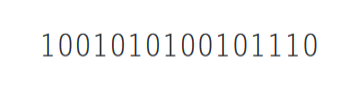
\includegraphics[width=10cm,height=3cm,keepaspectratio=false]{imagens-teoria/os_bits.png}
		
	\end{center}
	
	A resposta é NÃO, pois esse conjunto de bits pode representar várias coisas como números e até mesmo uma instrução, por exemplo.
	
	Uma instrução é um código binário que diz a CPU o que ela deve fazer, como somar um número, por exemplo.
	
	Isso acontece porque TODOS os computadores utilizam a Arquitetura de Von Neumann (veremos ela em detalhes posteriormente)

	\begin{center}
		
		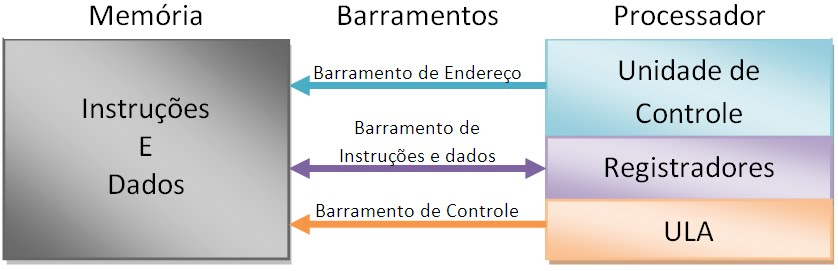
\includegraphics[width=11cm,height=4cm,keepaspectratio=false]{imagens-teoria/von-neumann.jpeg}
		
	\end{center}


	A arquitetura de Von Neumann faz com que a CPU converse com uma e apenas uma memória (a memória RAM) e assim, use a mesma representação (códigos binários) para dados (numeros, caracteres e etc) e instruções.
	
	Anteriormente, a arquitetura usada era a Havard, onde os dados e instruções ficavam em memórias separadas. Veja a baixo:
	
	\begin{center}
		
		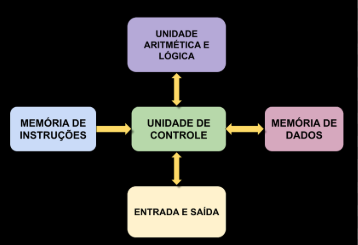
\includegraphics[width=9cm,height=4cm,keepaspectratio=false]{imagens-teoria/havard.png}
		
	\end{center}
	
	Inclusive, uma observação que é importante de ser feita é que o arduino utiliza a arquitetura de Havard, sendo que a memória das instruções é chamada de memória Flash ROM (contém 32KiB ), a memória que contém os dados é chamado de SRAM (contém 2KiB) e temos também uma memória que é tipo o disco rígido, chamada de EEPROM (contém 1KiB).
	
	\subsection{O programa e a maquina}
	
	Sabendo que o computador funciona em binário para tudo (instruções e dados), quando escrevemos nosso programa, ele precisa ir para o binário para que o computador possa entende-lo. Com isso nós temos algumas etapas:
	
	\begin{itemize}
		
		\item Linguagem de alto nível: A linguagem de alto nível será a linguagem que utilizamos em um geral, são aquelas que podemos compreender com facilidade (vamos utilizar o C para nossa explicação). Uma coisa importantissima nessa camada é o compilador, pois ele irá ler a linguagem e gerar o Assembly correspondente.
	\end{itemize}
	
	\begin{itemize}
		\item Assembly: O Assembly é uma camada meio que intemediária (pois abaixo dele ainda temos o assembler) e é ele irá fazer a ligação entre o software e o hardware. O assembly é uma linguagem formada pelas representações simbólicas das instruções. Essas representações simbólicas são palavras chave que a CPU entende (add, ld, sd). Uma curiosidade é que não podemos rodar um programa compilado em Intel para MAC, pois as palavras chaves do assembly são diferentes nas duas arquiteturas
		
		\begin{center}
			
			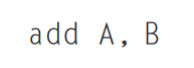
\includegraphics[width=6cm,height=3cm,keepaspectratio=false]{imagens-teoria/assembly.png}
			
		\end{center}
		
		Os compiladores possibilitaram nós de não precisarmos saber assembly de cada arquitetura. Isso acontece porque quando escrevemos nosso programa no alto nível, o compilador sabe o assembly de cada arquitetura.
	\end{itemize}
	
	\begin{itemize}
		\item Assembler: É a última camada. Ele lê as instruções Assembly e passa para binário para que o computador entenda.
		
		\begin{center}
			
			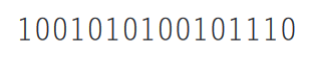
\includegraphics[width=7cm,height=2cm,keepaspectratio=false]{imagens-teoria/assembler.png}
			
		\end{center}
	\end{itemize}
	
	Entendido isso quando nós fazemos um Hello, World qualquer, nós temos:
	
	Codigo - Ola.c - Pre-processamento (Ola.i) - Assembly - Assembler
	
	\chapter{Parte 2}
	
	\section{Por debaixo dos panos}
	
	Algo que precisamos falar é: O que faz um computador ser um computador? Para ser um computador precisamos de: Input, Output, Memoria, Controle e Datapath. São esses componentes que definem o que chamamos de computador.
	
	\begin{center}
		
		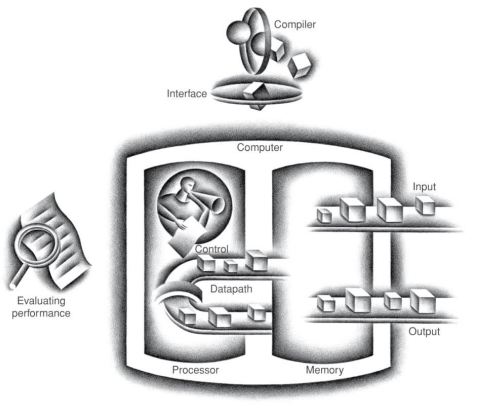
\includegraphics[width=12cm,height=10cm,keepaspectratio=false]{imagens-teoria/comp.png}
		
	\end{center}
	
	\begin{itemize}
		\item Datapath: Componente do processador que realiza operações aritméticas; circuitos para mover dados
		\item Controle: Componente do processador que comanda o datapath, memória e dispositivos de I/O, de acordo com as instruções de um programa
		\item Memória: Área de armazenamento na qual os programas são mantidos enquanto estão rodando. Contém: INSTRUÇÕES + DADOS
	\end{itemize}
	
	Um detalhe é que a nossa CPU (processador) é igual ao Controle + Datapath. O fluxo é:
	
	\begin{center}
		
		
\includegraphics[width=12cm,height=1cm,keepaspectratio=false]{imagens-teoria/cpu.png}
		
	\end{center}
	
	obs: a cpu buscará a instrução já em binário
	
	\subsubsection{Aprofundando o datapath}
	O datapath incluirá:
	
	\begin{itemize}
		\item Unidade Lógica e Aritmética (ALU): É o coração do Datapath, responsável por executar todas as operações matemáticas (adição, subtração) e lógicas (E, OU, NÃO).
		\item egistradores: Um pequeno conjunto de memórias de altíssima velocidade (ainda mais rápida que a L1 Cache) usadas para armazenar dados temporários, como os operandos (os números que estão sendo calculados) e resultados intermediários.
		\item 
		
	\end{itemize}
	
	Assim, o que acontece é que quando temos a instrução de somar X e Y, por exemplo, o que acontecerá será que o Controle irá buscar e pegar essa instrução, decodificar e guardar os valores na memória registradora. Esses valores serão jogados na ULA do nosso Datapath e irá realizar o calculo. Feito isso, o resultado sai da ULA e volta para o Datapath e joga nos registradores novamente.
	
	\subsection{Diferença ente microcontrolador e microprocessador}
	
	Microprocessador é aquilo que conhecemos. Ele precisa estar integrado à placa mâe e só faz operações logicas e aritmeticas (é o controle + datapath), por isso é rapido (4MHz). Tudo é exerno a ele.
	
	Nos microcontroladores, estamos falando de um minicomputador. Ele é tudo: controle + datapath, inputm output, ram, epprom...
	
	Uma curiosidade é que o microcontrolador do arduino UNO é chamado de ATMEGA328P-PU e sua arquitetura tem 8 bits.
	
	\subsection{Os monitores LCD do computador}
	
	\subsubsection{Funcionamento}
	
	Os monitores do computador são LCD (display de cristal liquido). O monitor é dividido em várias camadas. Veja abaixo:
	
	\begin{center}
		
		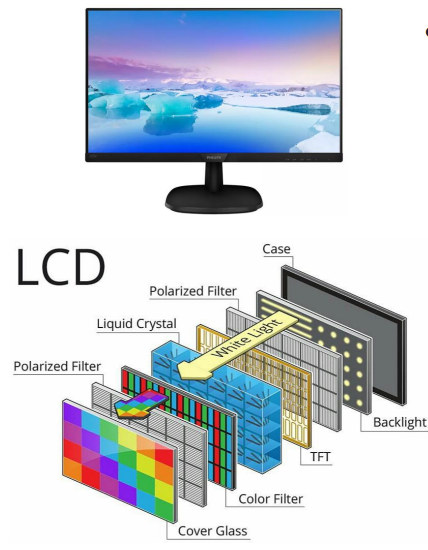
\includegraphics[width=12cm,height=10cm,keepaspectratio=false]{imagens-teoria/monitor.png}
		
	\end{center}
	
	Nós temos: o plastico (case), o painel de luz, o filtro polarizador (permite a passagem de luz branca em apenas uma direção), placa de cristal liquido (serve para mudar a angulação do raio de luz que ele recebe para passar no segundo polarizador), placa de cor (onde temos 3 transistors para cada pixel, cada um com 8 bits (RGB) e um segundo filtro polarizador
	
	O funcionamento acontece da seguinte forma: 
	
	\begin{enumerate}
		\item Imagine que a luz branca vinda do backlight (a lanterna da tela) está vibrando em todas as direções (horizontal, vertical, diagonal).
		\begin{itemize}
			\item O primeiro filtro polarizador (o de entrada) é colocado logo após o backlight.
			\item Ele só permite que a luz que vibra em uma única direção (por exemplo, vertical) passe.
			\item Toda a outra luz (que vibra nas outras direções) é bloqueada.
		\end{itemize}
		A luz que passa está agora polarizada (alinhada).
		
		\item A luz polarizada (vertical) entra na camada de cristais líquidos.
		\begin{itemize}
			\item Quando o pixel está desligado (sem eletricidade), os cristais torcem a luz em 90 graus (de vertical para horizontal, por exemplo).
		\end{itemize}
		
		
		
	\end{enumerate}
	
	A luz branca passa por uma camada de material especial: os cristais líquidos. Essas moléculas têm uma propriedade mágica: quando a eletricidade é aplicada a elas, elas se alinham ou torcem. Esse alinhamento é o que funciona como o "portão", pois com eletricidade, o cristal se torce e bloqueia a passagem da luz, criando o ponto preto na tela e sem eletricidade, o cristal se alinha de forma que a luz passa, criando o ponto branco.
	
	
	\subsubsection{Curiosidade}
	
	Uma curiosidade é que toda imagem que vemos em nossa tela é montada na memória em uma parte da memória chamada de Frame buffer, que armazena temporariamente os dados completos da imagem (os valores de cor e transparência de cada pixel) que será exibida na tela.
	
	Veja o funcionamento de forma detalhada:
	
	\begin{enumerate}
		\item Renderização (Criação dos Dados)
		Esta é a etapa onde a GPU (Placa Gráfica) trabalha.
		
		\begin{itemize}
			\item O software (jogo, navegador, etc.) envia os comandos para a GPU desenhar objetos 3D ou 2D.
			
			\item A GPU realiza os cálculos de geometria, aplica texturas, sombreamento e iluminação (processo conhecido como pipeline gráfico).
			\item O resultado final desse cálculo é a cor exata que cada pixel da tela deverá receber e exibir na tela.
			
		\end{itemize}
		A partir disso a informação de cor é transformada em uma sequência de bits. para cada pixel da nossa tela
		
		\begin{itemize}
			\item Lembrando que  a cor de um pixel é representada por 24 bits. Oito bits representam a intensidade do vermelho (R), oito a do verde (G) e oito a do azul (B) (RGB).
			\item Essa sequencia de bits é o que define a cor final. Por exemplo, a cor pura Vermelha pode ser representada por 11111111 00000000 00000000 (255 de Vermelho, 0 de Verde, 0 de Azul).
		\end{itemize}
		
		\item Armazenamento no Frame Buffer e montagem na tela
		\begin{itemize}
			\item O frame buffer  irá pegar as sequências de bits de cada pixel e armazenar isso. Ele é o estoque final da imagem.
			\item A partir disso, O Controlador de Vídeo (um componente de hardware) é quem lê o Frame Buffer, pegando as sequências de bits. Ele envia essa informação (pixel por pixel, linha por linha, numa cadência contínua chamada de taxa de refresh) para o monitor.
		\end{itemize}
		Algo interessante é que a taxa de refresh será quantas vezes o computado consegue recriar a imagem na tela por segundo. Sãs os Hz do monitor (60Hz, 144Hz)
	\end{enumerate}
	
	
	\subsubsection{Os tipos de touchscreen}
	
	Nos monitores, nós temos diferentes tipos de touchscreen. São eles:
	
	\begin{itemize}
		\item Resistivos: Precisam de pressão. São mais baratos e são muito utilizados em totens de pedidos ou de informações em shoppings, por exemplo
		\item Capacitivo: São sensíveis à distorções do campo eletromagnético da tela. São mais caros e são utilizados em telas de smartphones, por exemplo.
	\end{itemize}
	
	
	\subsection{A memória}
	\subsubsection{Sobre}
	A memória é uma hierarquia, onde temos:
	
	\begin{itemize}
		\item Memória Primária (ou principal)
		\begin{itemize}
			\item Armazena programas (dados e instruções) enquanto estãoem execução. É memória VOLÁTIL.
			\item DRAM, SRAM, ...
		\end{itemize}
		\item Memória secundária
		\begin{itemize}
			\item Memória NÃO VOLÁTIL usada para armazenamento de longo prazo (enquanto o computador está desligado).
			\item HD, flash memory, CD-ROM, ...
		\end{itemize}
	\end{itemize}
	
	Sabendo disso, essa hierarquia se apresenta da seguinte forma para nós:
	
	\begin{center}
		
		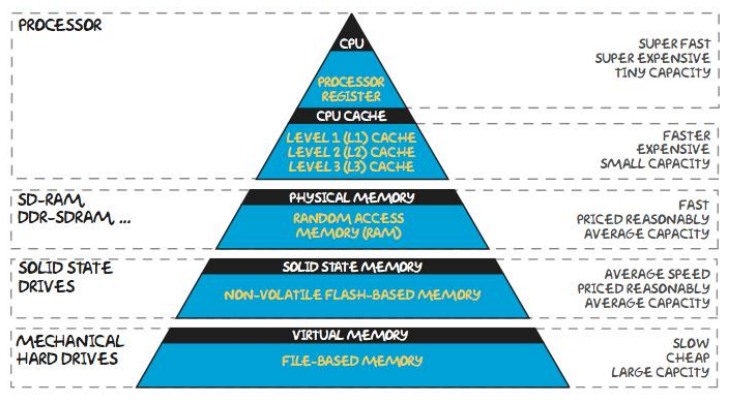
\includegraphics[width=9cm,height=7cm,keepaspectratio=false]{imagens-teoria/hierarquia_memoria2.png}
		
		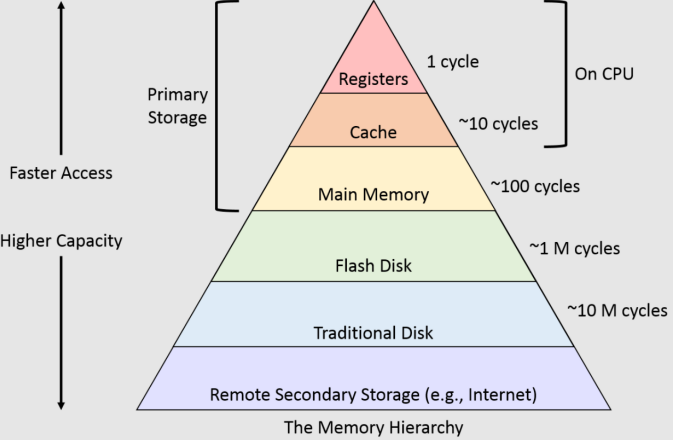
\includegraphics[width=9cm,height=7cm,keepaspectratio=false]{imagens-teoria/hierarquia_memoria3.png}
	\end{center}
	

	
	
	
	\subsubsection{Como funciona os transistors?}
	Certo, falamos disso tudo, mas como os transistors irão funcionar por dentro? Veja primeiramente a imagem abaixo:
	
	\begin{center}
		
		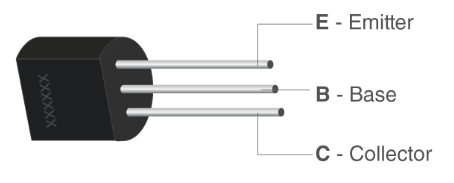
\includegraphics[width=6cm,height=4cm,keepaspectratio=false]{imagens-teoria/transistor1.png}
		
	\end{center}
	
	
	
	Acima, nós temos a imagem de um transistor. Ele terá três pernas: A da esquerda, chamada de coletor, a do meio, chamada de base e a da direita, chamada de emissor
	
	O coletor é por onde a corrente elétrica entra. A energia elétrica não saíra pela base, ela saírá pelo emissor.
	
	Para fazer a energia elétrica sair, usamos o silício, que é um semicondutor onde podemos controlar sua condutividade por conta das impurezas jogadas nele. Dentro do transistor, teremos o silício negativamente carregado "N" e o positivamente carregado "P". Normalmente o silicio positivamente carregado fica no centro, na região onde fica o pino da base e o silicio negativamente carregado fica ao redor.
	
	
	A base, poderá ficar positiva e negativa. Quando fica positiva, ela atrai as cargas negativas (elétrons) que estão nas regiões vizinhas do silício (os silicios tipo "N", que são negativamente carregados). Esses elétrons atraídos irão se acumular no silicio positivamente carregado (P) e fazer com que ele fique negativamente carregado (N), formando uma espécie de ponte, fazendo com que a eletricidade consiga fluir para o emisssor. Veja a imagem abaixo:
	
	\begin{center}
		
		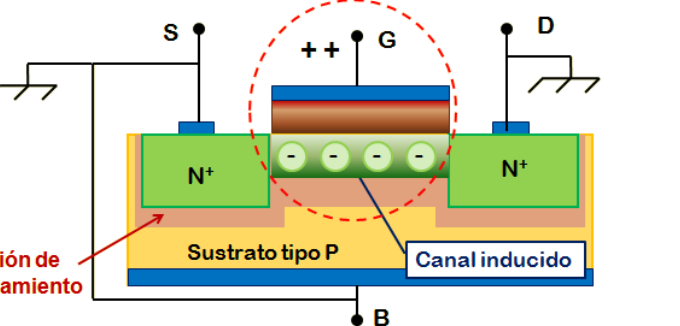
\includegraphics[width=8cm,height=4cm,keepaspectratio=false]{imagens-teoria/transistor2.png}
		
	\end{center}
	
	
	Para impedir novamente a passagem de eletricidade, colocamos a base do transistor como negativa, que irá repelir os elétrons e tornar o nosso silicio em positivamente carregado novamente, fazendo com que a ponte que se formou seja desformada, impedindo novamente a passagem de energia. 
	
	O computador normalmente tem por volta de 2,46GHz, o que siginifica que o transistor faz esse processo dentro dele por volta de 3 bilhoes de vezes por segundo.
	
	Uma curiosidade que a litografia é uma prática para tornar o tamanho da ponte (medida em nanometros) cada vez menor, pois quanto menor o tamanho dessa ponte, mais rápido ela forma e desforma (abre e fecha)
	
	\subsubsection{Como contruir processadores e memórias}
	
	\begin{center}
		
		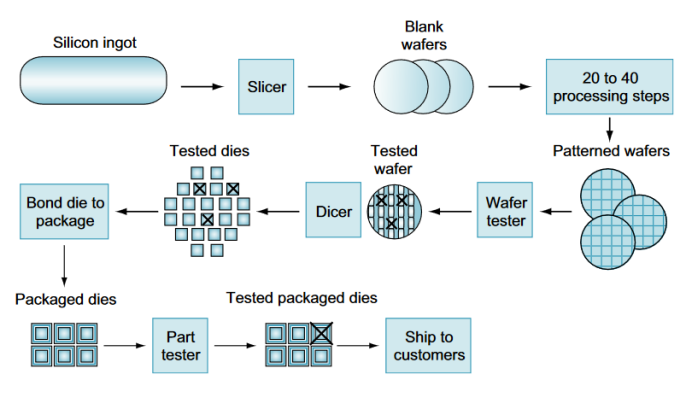
\includegraphics[width=9cm,height=5cm,keepaspectratio=false]{imagens-teoria/construir_process.png}
		
	\end{center}
	
	\chapter{Sobre Perfomance dos Computadores}
	
	\section{Qual a definição?}
	A definição de performance de um computador é um pouco dificil de ser medida, pois depende do ponto de vista que formos usar: projetista e usuario.
	
	Isso é complicado, pois nem sempre ambos os pontos de vista serão coincidadentes. O usuario não esta interessadp na ideia de performance do projetista da cpu.
	
	\chapter{Sobre os processadores}
	
	\section{Como funcionam?}
	Para entender como os processadores funcionam, precisamos primeiro entender qual é a função deles. A função do processador é, a partir de instruções, mandar o hardware fazer algo (somar 2 +2, por exemplo).
	
	
	Um exemplo que já falamos no incio desse documento e que nos ajudar a entender um pouco é quando temos nosso programa que faz a soma de dois números. Veja abaixo:
	
	
	O código acima é a ação que mandamos a cpu executar em alto nivel. É a nossa sentença. O compilador transforma (a grosso modo) sentenças em instruções e as instruções, como sabemos, é o binário que a CPU entende e executa. 
	
	É importante ressaltar que a CPU SÓ ENTENDE BINÁRIO, sendo que cada arquitetura (86\_64, RISC-V, ARM) entende as instruções (binários) de uma maneira diferente para a mesma ação. Exemplo: A instrução (binario) soma é diferente para diferentes arquiteturas e, como ja vimos anteriormente, esse é o motivo pelo qual não pegamos um programa compilado no processador de arquitetura intel para roda no macbook (arquitetura ARM).
	
	\section{Aprofundando}
	O conjunto das palavras (instruções) que cada processador usa é chamado de ISA, portanto, no fim das contas, quem faz o meio campo entre o nosso programa (alto nivel) e a CPU é a ISA
	
	
	
	\section{Funcionamento da CPU}
	
	\subsection{Nome aos bois}
	
	Na CPU nós teremos os registradores de uso geral e os registradores especiais (além das outras coisas como memória RAM, mas para entender, nos importará essas). Dentre os registradores especiais nós temos:
	
	\begin{itemize}
		\item R.I (registrador de instrução): Aponta para a instrução que está sendo executada
		\item C.P: Aponta para a próxima instrução a ser executada 
	\end{itemize}
	
	\subsection{Funcionamento de fato}
	
	Para entendermos o funcionamento, temos que ter em mente que na arquitetura Von Neumann (a arquitetura dos computadores modernos), memória e instruções ficam na mesma memória, com a mesma representação (binários)
	
	Entendido isso, quando nós temos um programa que faz a soma de dois números, nós teremos, na memória RAM os dados e também as intruções. Ao executar, o sistema operacional pega a pimeira instrução e leva ao C.P. e depois joga para R.I e C.P irá apontar para a próxima instrução. RI executa a instrução que estava lá para que C.P jogue a instrução que estava lá para apontar para a proxima. Isso ocorre até o fim do programa.
	
	\subsection{Um detalhe}
	
	Certo, falamos anteriormente como funciona o funcionamento, mas algo que temos que falar é que a CPU não consegue ir na memória RAM e realizar a soma lá na memória. A CPU não atua diretamente na memória, ela carrega os dados da memória nos registradores, faz a conta e retorna o resultado na memória
	
	Um exemplo disso que vimos é no assembly, quando utilizamos o ADD, por exemplo. Nós teremos o operador e mais 3 coisas, sendo que a primeira coisa é o registrador de destino (depois de fazer a soma, o resultado será colocado no registrador de destino), o registrador fonte 1 e o registrador fonte 2, onde teremos o conteúdo que veio da memória para que nós fizessemos a soma. Com o resultado da soma no registrador de destino, esse resultado vai para a memória RAM
	
	
	O operador que irá buscar o conteúdo da RAM e colocar nos registradores é chamado de LW (load word)
	
	Nas leituras de memória, ao utilizar o operador LW, temos o REB que é registrador que contem o ENDEREÇO BASE de uma variavel (o endereço base é onde aquilo começa na memória), depois temos o OFFSET, que é o deslocamento necessário para alcançar o dado desejado e depois o RD, que é o registrador de destino, onde iremos guardar o dado desejado.
	
	\subsubsection{Exemplo}
	Para entender melhor, vamos a um exemplo: Suponhamos que na memória nós tenhamos um array={1,101,10,100}. Se quisermos carregar o elemento A[2] (10) no registrador x3, fazemos:
	
	\begin{center}
		\begin{LARGE}
			LW x3 2 64
		\end{LARGE}
	\end{center}
	
	Olhando acima, da direita para a esquerda, nós temos o endereço base desse array (o endereço base será o compilador que irá definir. Quando o compilador gera as instruções, ele coloca o endereço base em algum registrador e forma isso no assembly), depois temos o deslocamento onde para chegar no elemento 10, nós andamos 2 (do 64 ao 66), e por fim o registrador de destino.
	
	Sendo assim, estamos dizendo: Carregue o dado no registrador x3 a partir do endereço base 64 com deslocamento 2.
	
	Um detalhe é que o exemplo acima que acabamos de explicar é um exemplo simplificado que não corresponde a realidade exatamente, pois cada célula é 1byte (8 bits) e um inteiro não coupa 1 célula, ocupa 4. Portanto, explicando de uma maneira mais fideldigna:
	
	\subsubsection{Big endian e Little endian}
	
	Algo que temos que falar, apesar de não ser tão importante é sobre o Big endian e o Little endian. Esses termos significam como armazenamos dados que precisam de mais de uma célula de memóra. Vamos definir cada um deles:
	
	\begin{itemize}
		\item Big endian:Byte mais significativo no menor endereço 
		\item Little endian: Byte mais significativo no maior endereço de memória (Byte menos significativo no mmenor endereço de memória)
	\end{itemize}
	
	É importante falarmos desse assunto porque ao usar a memória EPROM, precisamos saber disso. O arduino é little endian (a intel também)
	
	\subsubsection{Falando do envio dos dados}
	
	Já falamos do uso do LW para enviar da memoria para os registradores. Agora, temos o caminho contrário. Para isso, utilizamos o operador SW, onde temos o REB que como já vimos é o registrador que contem o ENDEREÇO BASE de uma variavel, o OFFSET 
	
	
	\subsection{O baixissimo nivel}
	
	Aprendemos como o compilador sai do alto nível e chega no assembly. Agora, temos que saber como sai do assembly para o binário
	
	Para isso, temos que saber que cada linha do assembly é uma instrução (uma linha de binário). Cada operação tem seu próprio formato. Exemplo:
	
	y = x + z. O assembly disso é: ADD x5 x4 x3. O binario disso será:
	
	
	
	De trás para frente, nós temos o OPCODE (reserva os 7 bits do final)  do operador ADD, que é 51 em binário
	
	
	Um detalhe é que todos os operadores terão seu próprio OPCODE, F3 e FUN7, que definirão qual operador será ele
	
	
\end{document}
